\section{9/10/2019}

Recall the planted clique from \cite{alon1998finding}: $G \sim G(1/2, n, k)$
is a random graph on $V = [n]$ with some fully connected
clique $K \subset [n]$ of cardinality $\lvert K \rvert = k$.

The adjacency matrix
\begin{align}
  A_{ij} &=
  \begin{cases}
    1 &\text{if }i,j \in K \\
    \text{Bern}(1/2) &\text{$i \neq j$ ow}
  \end{cases}
\end{align}

Let
\begin{align}
    W_{ij} &= \begin{cases}
        2 A_{ij} &\text{if }i \neq j \\
        0 &\text{if }i = j
    \end{cases}
\end{align}
Algorithm 1 of \cite{alon1998finding}:
\begin{enumerate}
    \item Find top eigenvector of $W$, say $u$
    \item Let $\tilde{K}$ index the largest $k$ coordinates $\lvert u_i \rvert$
    \item Define $\hat{K} = \{ v \in V : d_{\tilde{K}}(v) \geq \frac{3 k}{4} \}$
\end{enumerate}

\begin{theorem}[\cite{alon1998finding}]
    Algorithm 1 finds $\hat{K}$ such that $\Pr[\hat{K} = K] \to 1$ as $n \to \infty$
    if $k \geq c \sqrt{n}$ for sufficiently large $c$.
\end{theorem}

\begin{proof}
    Note that $\ex A$ is:
    \begin{figure}[H]
        \centering
        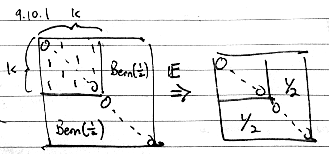
\includegraphics[width=0.6\textwidth]{figures/9-10-1.png}
        \caption{$\ex A$ has ones in the upper $k \times k$ block,
            $0$ on the diagonal, and $1/2$ everywhere else}
    \end{figure}
    
    From this, we can easily see that the $\ex W$ is:
    \begin{figure}[H]
        \centering
        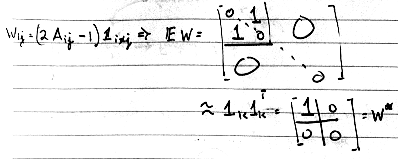
\includegraphics[width=0.6\textwidth]{figures/9-10-2.png}
        \caption{$\ex W$ differs from $W^* = 1_k 1_k^\top$ only in the upper $k$ diagonal}
    \end{figure}
    Note $\ex W = 1_K 1_K^\top - \diag(1_K) \approx 1_K 1_K^\top = W^*$, which
    is good because we have seen that ``differenes in the diagonal are asymptotically negligible.'' \todo{reference for this? 9-5 lecture}
    
    \textbf{Goal}: show $\lvert \tilde{K} \cap K \rvert \geq (1 - \eps) k$ whp, $\eps = \eps(c)$.
    
    We first show the top eigenvector of $W^*$ is close
    to $u$ (the top eigenvector of $W$).
    Let $v = \frac{1}{\sqrt{k}} 1_K$ be the top eigenvector of $W^*$.
    Note $\lambda_1(W^*) = k$.
    By Davis-Kahan
    \begin{align}
        \min_{s \in \{\pm 1\}} \|u + s v\|_2
        &\leq \frac{\|W - W^*\|_{2}}{\lambda_1(w^*) - \lambda_2(w)}
    \end{align}
    Note
    \begin{align}
        \|W - W^*\|
        &\leq \|W - \ex W\| + \|\ex W - W^* \|
        \leq c \sqrt{n} + 1
    \end{align}
    Also $\lambda_1(W^*) = k$ and
    \begin{align}
        \lvert \lambda_2(W) \rvert
        &\leq \lvert \lambda_2(W^*) - \lambda_2(W)
        \leq \|W^* - W\|
    \end{align}
    So by Weyl's inequality
    \begin{align}
        \min_{s \in \{\pm 1\}} \|u + s v\|_2
        &\leq \frac{c \sqrt{n} + 1}{ k - (c \sqrt{n} + 1)} \\
        &\leq \frac{c \sqrt{n} + 1}{c \sqrt{n} - c \sqrt{n} + 1}
        \leq \eps
    \end{align}
        
    Aside: Davis-Kahan to get bound between difference of eigenvectors in 2-norm. Open problem
    to control others.
    
    Next, if $\lvert K \rvert = k = \lvert \tilde{K} \rvert$ then
    $\lvert K \setminus \tilde{K}\rvert = \lvert \tilde{K} \setminus K \rvert$.
    
    \begin{figure}[H]
        \centering
        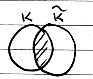
\includegraphics[width=0.2\textwidth]{figures/9-10-3.png}
        \caption{$\lvert K \rvert = \lvert \tilde{K} \rvert \implies \lvert K \setminus \tilde{K} \rvert = \lvert \tilde{K} \setminus K \rvert$ follows from elementary set theory}
    \end{figure}
    
    By definition of $v$
    \begin{align}
        \eps^2
        \geq \|u - v\|_2^2
        = \sum_{i \in K} (u_i - \frac{1}{\sqrt{k}})^2 + \sum_{i \not\in K} u_i^2
    \end{align}
    
    \begin{lemma}
        If all $\lvert u_i \rvert \leq \frac{1}{2 \sqrt{k}}$ for $i \not\in \tilde{K}$, 
        then
        \begin{align}
            \eps^2 
            \geq \sum_{i \in K \setminus \tilde{K}} (\frac{1}{\sqrt{k}} - u_i)^{2} 
            \geq \sum_{i \in K \setminus \tilde{K}} \frac{1}{4k}
        \end{align}
        This implies $\lvert K \setminus \tilde{K} \rvert \leq 4 \eps^2 k$.
    \end{lemma}
    
    \begin{lemma}
        If the condition of the previous lemma does not hold, then $\exists i \in \tilde{K}$
        with $\lvert u_i \rvert \geq \frac{1}{2 \sqrt{k}}$. Then in fact $\lvert u_i \rvert \geq \frac{1}{2 \sqrt{k}}$ for all $i \in \tilde{K}$ since
        \begin{align}
            \eps^2
            &\geq \sum_{i \in \tilde{K} \setminus K} u_i^2
            \geq \sum_{i \in \tilde{K} \setminus K} (\frac{1}{2 \sqrt{k}})^2
            = \sum_{i \in \tilde{K} \setminus K} \frac{1}{4k}
        \end{align}
        Hence $\lvert \tilde{K} \setminus K \rvert \leq 4 \eps^2 k$
    \end{lemma}
    So we have achieved our goal.
    
    To finish the proof, first assume $\|u - v\|_2 \leq \eps$.
    For $a \in K$,
    \begin{align}
        d_{\tilde{K}}(a)
        \geq d_{\tilde{K} \cap K}(a)
        = \lvert \tilde{K} \cap K \rvert - 1
        \geq (1 - \eps') k
    \end{align}
    so for $a \in K$, we will get $a \in \hat{K}$.
    
    Now if $a \not\in K$,
    \begin{align}
        d_{\tilde{K}}(a)
        \leq \underbrace{d_K(a)}_{\sim \text{Binom}(k, 1/2)} + \underbrace{\lvert \tilde{K} \setminus K \rvert}_{\leq \eps' k}
        \approx \frac{k}{2} \pm c \sqrt{k}
    \end{align}
    where $\approx$ means concentration. To be concrete,
    \begin{align}
        \Pr[\hat{K} \neq K]
        &\leq \Pr[\|u - v\|_2 \geq t]
        + \Pr[\exists a \not\in K : d_K(a) \geq (\frac{3}{4} - \eps') k] \\
        &\leq \Pr[ \|W - \ex W\| \geq c \sqrt{n} ]
        + (n - k) \Pr[B(k, 1/2) \geq (\frac{3}{4} - \eps) k] \\
        &\leq c e^{-c' n} + (n - k)
    \end{align}
    
    Where above we used the multiplicative version of Chernoff bound 
    (useful in combinatorial statistics):
    \begin{lemma}[Multiplicative Chernoff Bound]\label{lem:mult-chernoff}
        \begin{align}
            \Pr[X \geq (1 + \delta) \mu]
            &\leq \begin{cases}
                e^{-\delta^2 \mu / 3} &\delta \in [0,1] \\
                e^{-\delta \mu / 3} &\delta \geq 1
            \end{cases} \\
            \Pr[X \leq (1 - \delta) \mu]
            &\leq e^{-\delta^2 \mu / 2}
        \end{align}
    \end{lemma}
    
    As $n \to \infty$, we see that $\Pr[\hat{K} = K] \to 1$.
\end{proof}

\cref{lem:mult-chernoff} is self-normalizing: let $X = \sum_{i=1}^n X_i$ with $X_i$ independent binary
and $\mu = \ex X$. Note that after applying, the RHS does not depend on $n$ \todo{Verify}


\textbf{AKS Algorithm 2}: This algorithm is designed to handle the case when $k$ is not big enough
(recall algorithm 1 requires $k \geq c \sqrt{n}$).
Search over all $S$ with $\lvert S \rvert = C(c) = 2 \log_2 \frac{10}{c} + 2$. For each $S$:
\begin{enumerate}
    \item Define $N^*(S) = \{ v \in V : v \sim a, \forall a \in S \} \setminus S$
    \item Run Algorithm 1 on the induced subgraph (which has distribution $G(1/2, N^*(S), K-S)$),
        return $Q_S \cup S$
    \item Output if $Q_S \cup S$ is a $k$-clique
\end{enumerate}

\textbf{Intuition}: Suppose $k=0$ so there's no clique. Then $\lvert N^*(S) \rvert \sim B(n-s, 2^{-s})
\approx \frac{n-s}{2^s}$ so the total number of nodes is much smaller (by order of $2^{-s}$).
However, the number of clique nodes in $N^*(S)$ is still relatively large, $\geq k - s$.
Solving the critical equation (also for algorithm 1 \todo{Track htis down})
\begin{align}
    k - s \geq C \sqrt{\frac{n}{2^s}}
\end{align}
yields the expression for $C(c)$.


\begin{theorem}
    As long as $k \geq (2 + \eps) \log_2 n$, then exhaustive search finds $k$
    with probability $\to 1$.
\end{theorem}

\begin{proof}
    Exhaustive search will always find the clique, but it may return a clique that we didn't plant.
    So we need to guarantee there is no clique of size $(2 + \eps) \log_2 n$ in $G$ whp.
    
    For $S \subset [n]$, $\lvert S \rvert = k$,
    \begin{align}
        \Pr[S~\text{is clique}] &= \frac{1}{2^{\binom{k}{2}}} \\
        \Pr[\exists S \subset [n] : S~\text{is clique}]
        &\leq \binom{n}{k} \frac{1}{2^{\binom{k}{2}}} 
        \leq (n 2^{-(k-1)/2})^k \to 0\\
    \end{align}
    as $n \to \infty$ ($k = (2 + \eps) \log_2 n$).
\end{proof}